% !TEX root = ../presentation.tex

\begin{frame}{Нормализация по пакету}
\begin{figure}
\centering
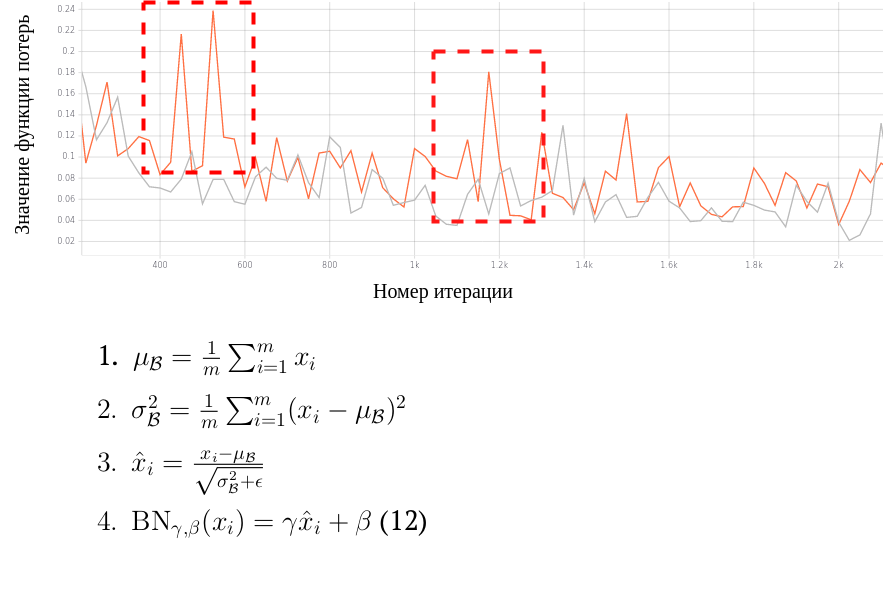
\includegraphics[width=9.11cm, height=6.50cm]{batch_normalization_pres.png}
\end{figure}
    Оранжевым цветом отражен процесс обучеения без нормализации, серым - с нормализацией.
%\textbf{$C$}-центр камеры (оптический центр); \textbf{$Cp$}-главная ось камеры
\end{frame}